\section{Etherless-server architecture}
\subsection{Architecture overview}
Etherless-server architecture is composed of two different modules:
\begin{itemize}
	\item Funcions
	\item Runner
\end{itemize}
\begin{figure}[!h]
\centering
	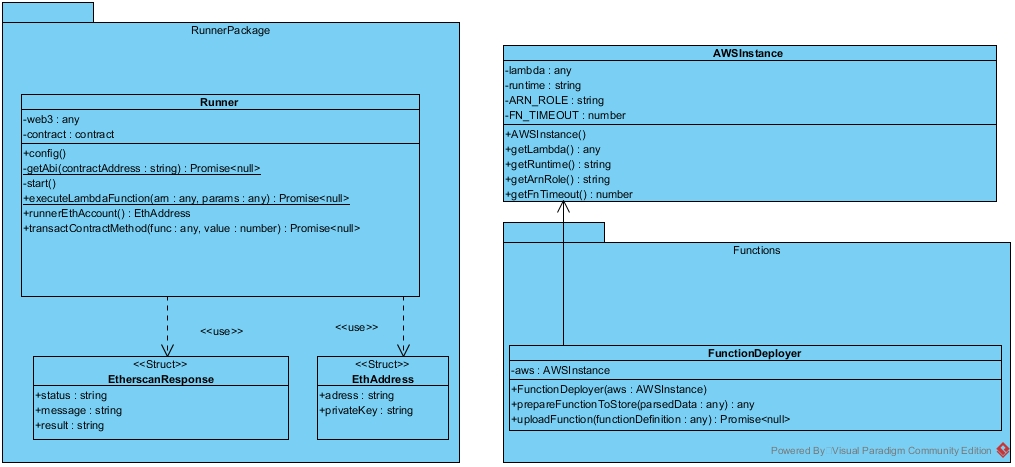
\includegraphics[width=\textwidth]{res/img/etherlessServer.jpg}
	\caption{Architecture overview of etherless-server}
\end{figure}
\subsubsection{Functions}
Functions module contains all the command functions which are stored on AWS Lambda. \\
In particular, here will be implemented three files corresponding these three following commands:
\begin{itemize}
	\item \textbf{createFunction (FunctionDeployer):} creates a new AWS Lambda function with the JavaScript resource uploaded by developer users from CLI\glo;
	\item \textbf{removeFunction:} deletes the corrisponding Lambda function on AWS Lambda;
	\item \textbf{updateFunction:} used to update the implementation of a function already deployed by a user on AWS Lambda.
\end{itemize}
All these three files depend on a class called "AWSInstance" containing all the informations about the execution environment of AWS Lambda:
\begin{itemize}
	\item \textbf{RUNTIME:} about Nodejs version of AWS environment;
	\item \textbf{ARN ROLE}
	\item \textbf{FN TIMEOUT:} about timeout given to function's execution.
\end{itemize}

\subsubsection{Runner}
This component runs persistently listening events from Smart Contract deployed on Ethereum\glo Network. Once the smart-contract \textit{ABI\glo} has been downloaded, Runner use the "executeLambdaFunction" method to run the corresponding Lambda function on AWS.\\ Runner component is deployed on AWS Elastic Beanstalks which reduces management complexity and allows to keep it always alive. 


\subsection{Methods}
\subsubsection{Runner}
\begin{itemize}
	\item \textbf{config:} Creates the smart-contract instance downloading the corresponding \textit{ABI\glo} and then calls start method;
	\item \textbf{start:} Start to listen Ethereum\glo events emitted by Etherless-smart, calls "executeLambdaFunctionMethod" to run the Lamdda requested and then returns the response;
	\item \textbf{getAbi:} retrieves and parses the smart-contract \textit{ABI\glo} from Etherscan;
	\item \textbf{executeLambdaFunction:} invoke the AWS Lambda function requested;
	\item \textbf{transactContractMethod:} calls a smart-contract method through a transaction.
\end{itemize}
\subsubsection{AWSInstance}
\begin{itemize}
	\item \textbf{getLambda:} returns a new AWS Lambda object
	\item \textbf{getRuntime:} returns the version of the AWS runtime;
	\item \textbf{getRole:} returns the AWS Lambda function's execution role;
	\item \textbf{getTimeout:} returns AWS Lambda function's \textit{timeout\glos}. 
\end{itemize}
\subsubsection{Runner}
\begin{itemize}
	\item \textbf{config:} Creates the smart-contract instance downloading the corresponding \textit{ABI\glo} and then calls start method;
	\item \textbf{start:} Start to listen Ethereum\glo events emitted by Etherless-smart, calls "executeLambdaFunctionMethod" to run the Lamdda requested and then returns the response;
	\item \textbf{getAbi:} retrieves and parses the smart-contract \textit{ABI\glo} from Etherscan;
	\item \textbf{executeLambdaFunction:} invoke the AWS Lambda function requested;
	\item \textbf{transactContractMethod:} calls a smart-contract method through a transaction.
\end{itemize}
\subsubsection{FunctionDeployer}
\begin{itemize}
	\item \textbf{createFunction:} calls prepareFunctionToStore and uploadFunction methods and then return the upload's result.
	\item \textbf{uploadFunction} upload effectively a file.js containing the user's function;
	
\end{itemize}
